
\includegraphics[height=1.5cm]{images/pictograms/tools}


\lstinputlisting[language=bash,basicstyle=\small]{python_codes/fieldstone_102/keywords.ascii}

\begin{center}
Code at \url{https://github.com/cedrict/fieldstone/tree/master/python_codes/fieldstone_102}
\end{center}

\par\noindent\rule{\textwidth}{0.4pt}

%%%%%%%%%%%%%%%%%%%%%%%%%%%%%%%%%%%%%%%%%%%%%%%%%%%%%%%%%%%%%%%%%%%%%%%%%%%%%%%%%%%%%%%%%%%%%%%%%%%%


\begin{center}
\includegraphics[width=1cm]{images/fortran/fortran} 
\end{center}

The topic of Conformal Mesh Refinement is introduced in Section~\ref{MMM-ss:cmr}.
This stone is a 'simple' approach to the implementation of Conformal Refinement. The code was written 
a few years prior to my working on fieldstone, so it is in Fortran. It is a 
simple Finite Element code which relies on $Q_1\times P_0$ elements. It solves the 
manufactured solution problem of Section~\ref{MMM-mms1}.

Let us start with a very simple test: the mesh counts $9\times 7=63$ elements.
The greyed elements are those to be refined. We then first flag 
the nodes which compose them and these are shown in teal color.
Based on this information we can then consider each element in the mesh and assign it a type, 
based on whether or not one or more nodes are flagged: 

\begin{center}
\input{tikz/tikz_cr_1}
\end{center}

The type is stored in the elemental array {\tt crtype} while the nodes belonging to elements 
to be refined are stored in {\tt crnode}.
There are 15 types of elements (the element type is tied to how many and which vertices are flagged nodes):

\begin{center}
\input{tikz/tikz_cr_2}
\end{center}

Note that the refinement above is based on a 3x3 refinement of elements. One could also carry out a 5x5-type
refinement which would then rely on the following elements (and their rotated versions)\footnote{I have never
seen a concrete example of these...}:
\begin{center}
\input{tikz/tikz_cr_3}
\end{center}

After running the code, various vtu files are to be found in the OUT folder.
{\filenamefont solution.vtu} contains the refined mesh with the calculated 
solution. 

\newpage
%................................................................
\paragraph{Case test=0}

The domain size is 9x7 and nelx=9, nely=7, so that all elements are square. 
The code solves the FE system but it is pointless as this test is about demonstrating 
the resulting mesh from the flagged elements at the beginning of this stone. 

\begin{center}
a)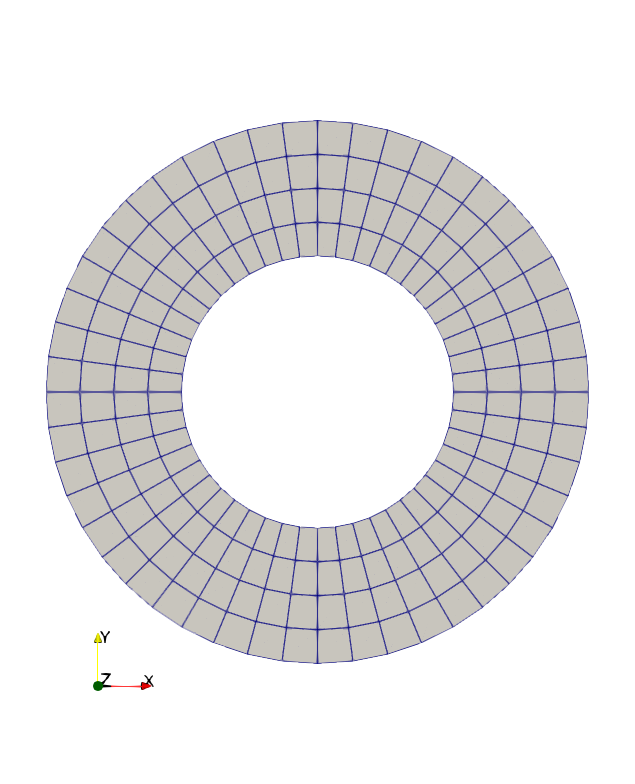
\includegraphics[width=7cm]{python_codes/fieldstone_102/results/test0/mesh1}
b)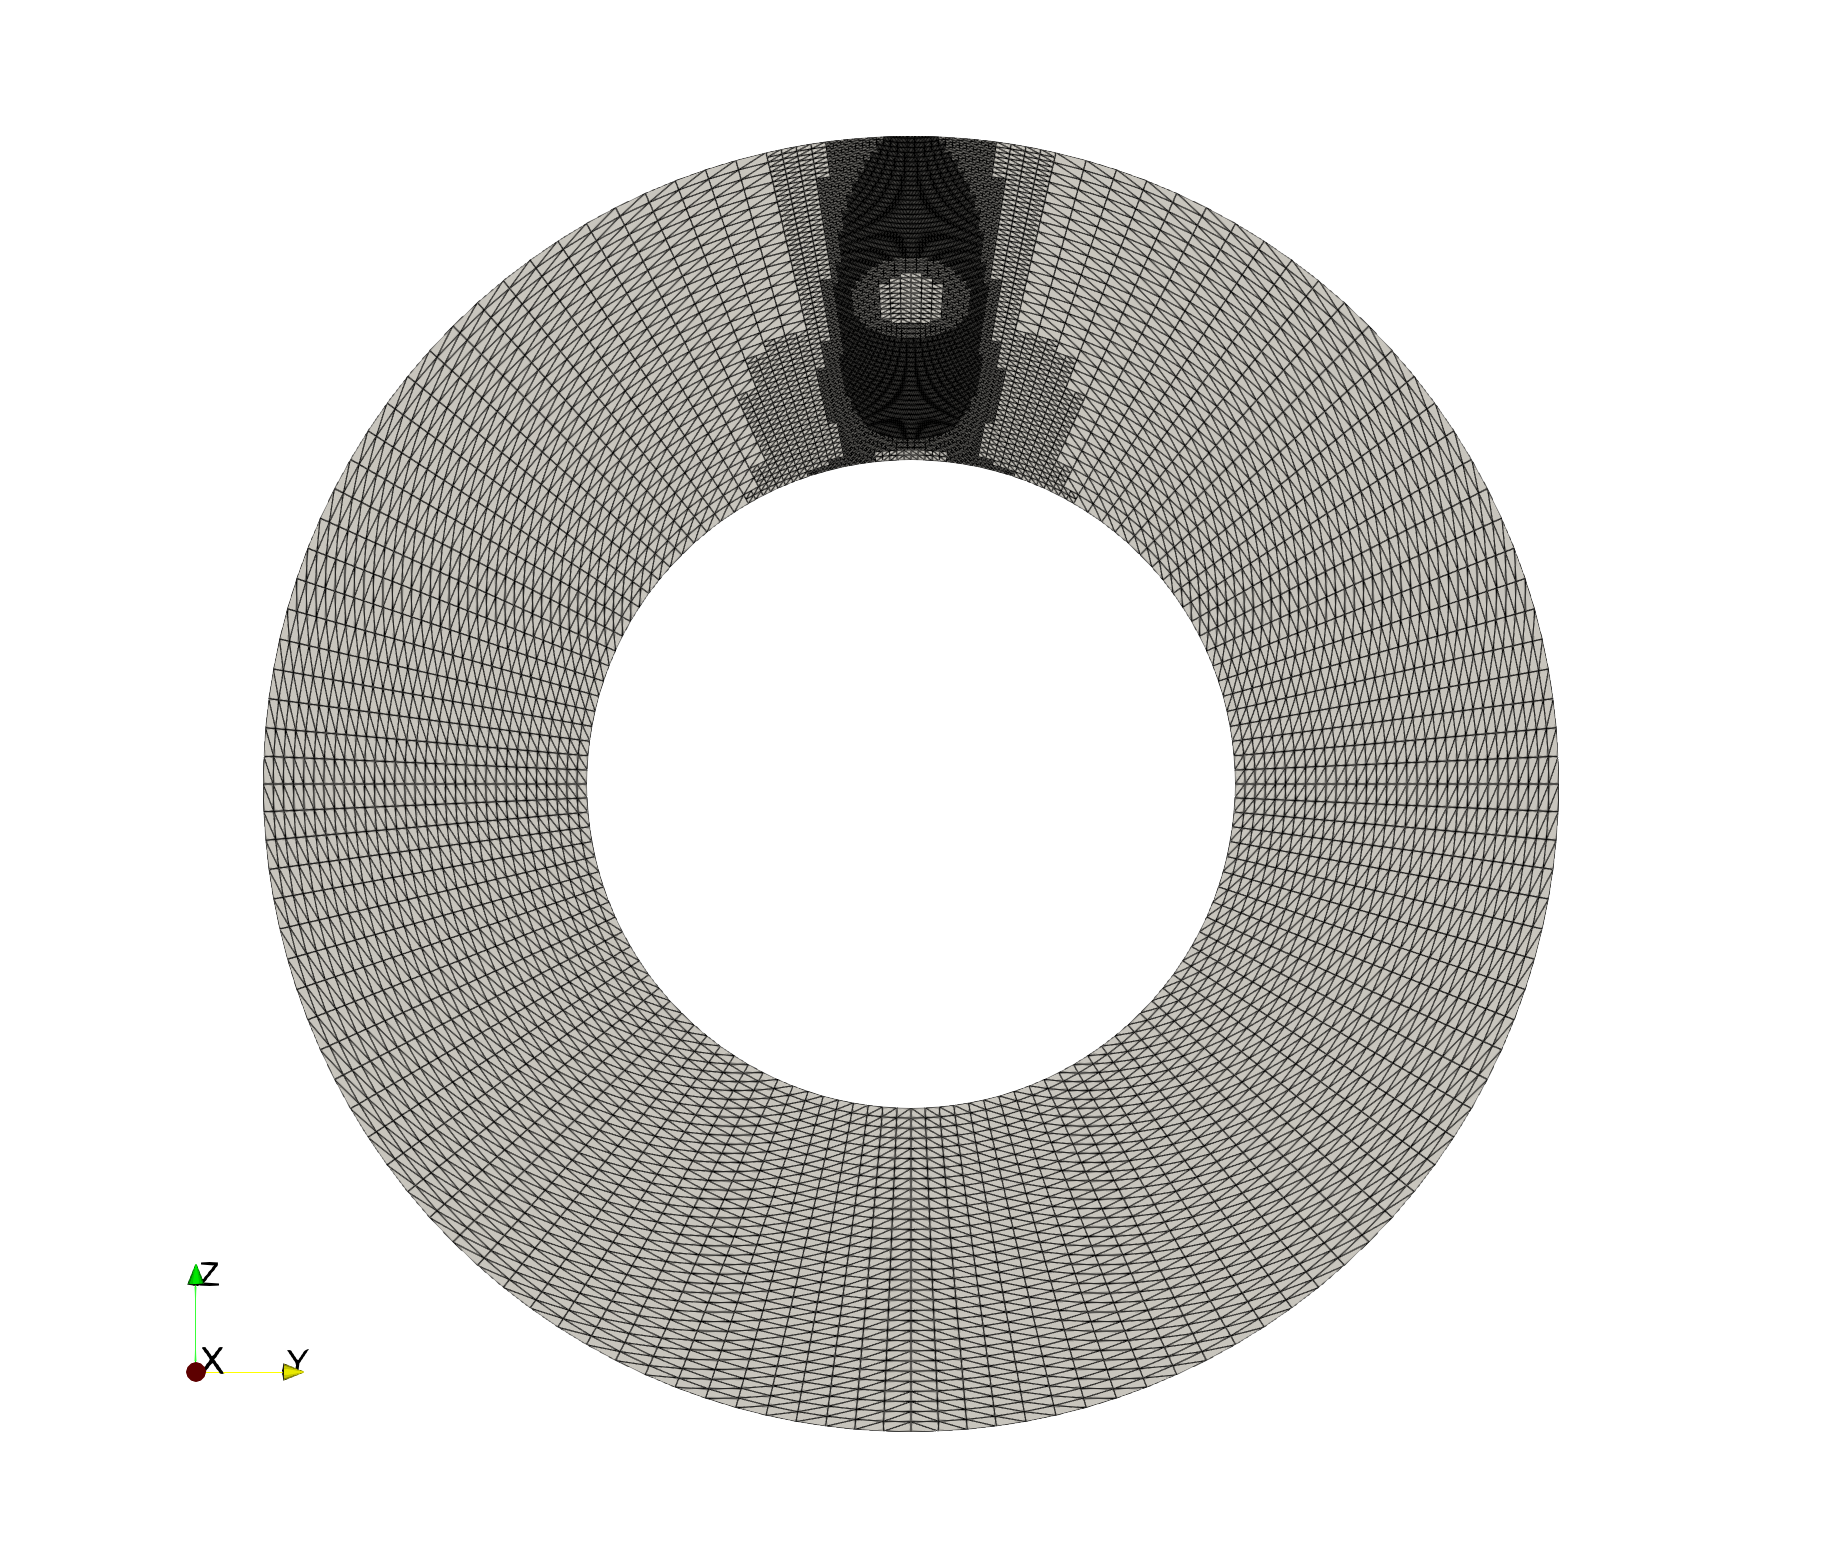
\includegraphics[width=7cm]{python_codes/fieldstone_102/results/test0/mesh2}\\
c)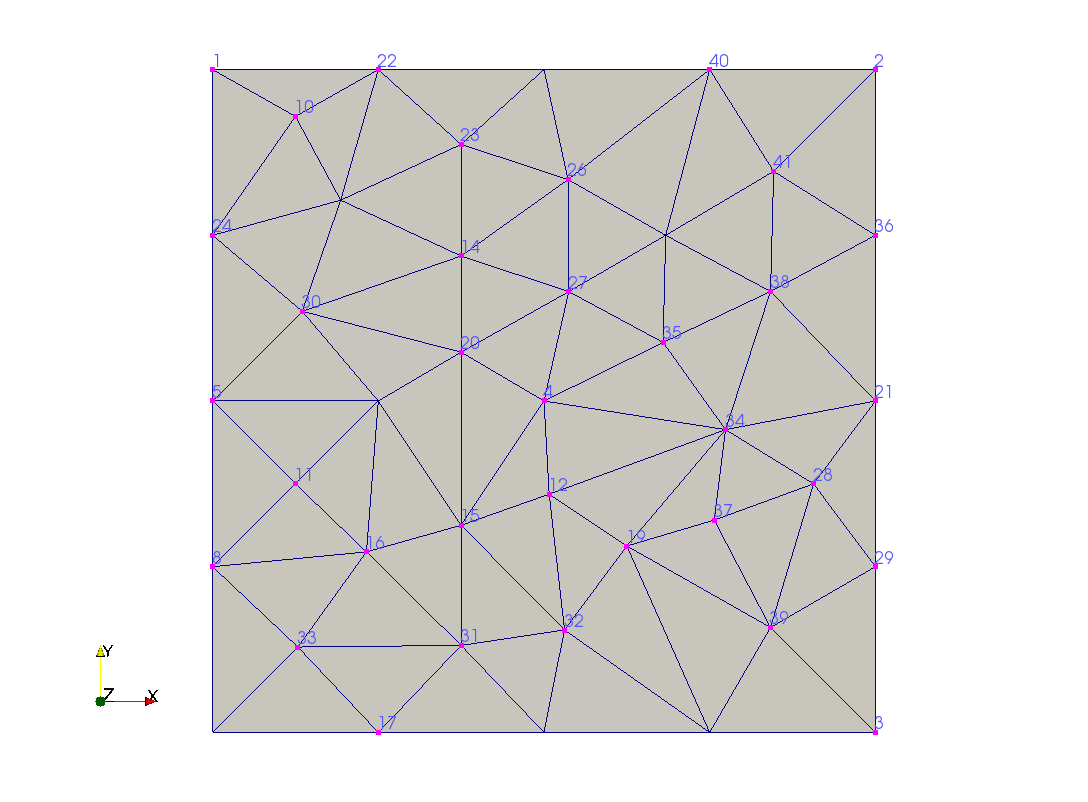
\includegraphics[width=7cm]{python_codes/fieldstone_102/results/test0/mesh3}
d)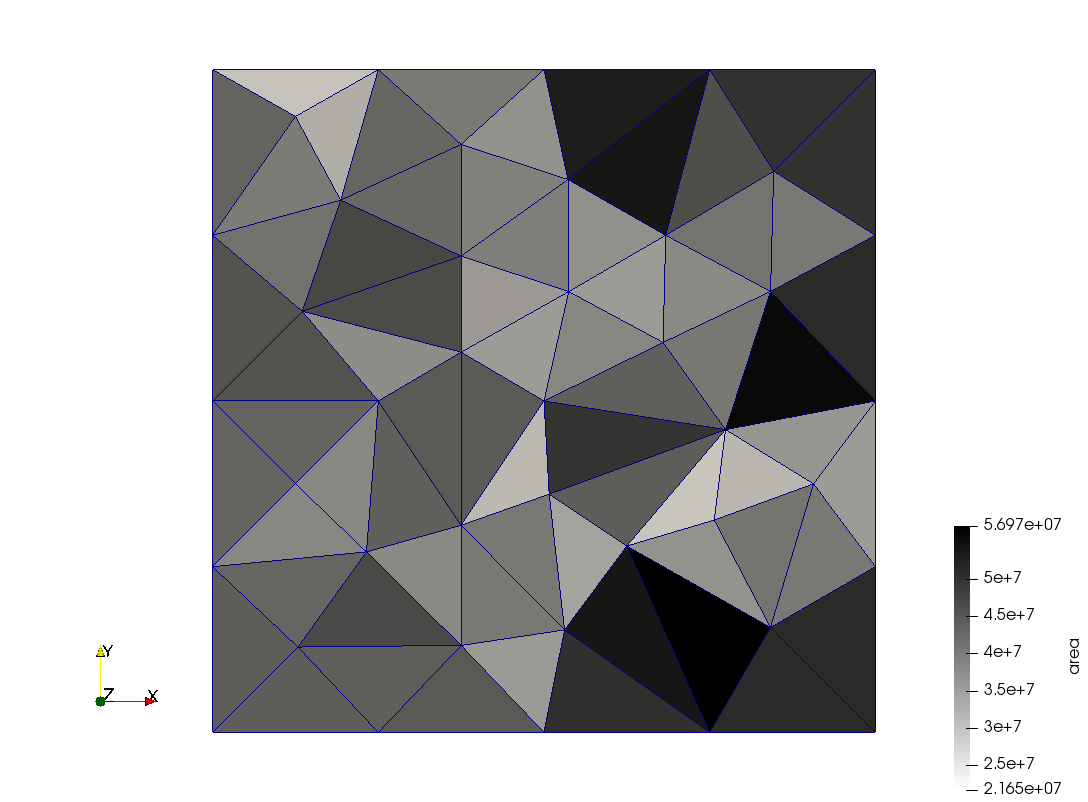
\includegraphics[width=7cm]{python_codes/fieldstone_102/results/test0/mesh4}\\
{\captionfont a) original mesh. b) flagged nodes. c) element types. d) refined mesh.}
\end{center}

%................................................................
\paragraph{Case test=1,2,3}

\begin{center}
\includegraphics[width=5.6cm]{python_codes/fieldstone_102/results/test1/vel}
\includegraphics[width=5.6cm]{python_codes/fieldstone_102/results/test2/vel}
\includegraphics[width=5.6cm]{python_codes/fieldstone_102/results/test3/vel}\\
\includegraphics[width=5.6cm]{python_codes/fieldstone_102/results/test1/press}
\includegraphics[width=5.6cm]{python_codes/fieldstone_102/results/test2/press}
\includegraphics[width=5.6cm]{python_codes/fieldstone_102/results/test3/press}\\
{\captionfont Initial resolution 10x10. 
Left: The left half of elements are flagged for refinement.
Middle: The elements above the diagonal are flagged for refinement.
Right: Every 7 elements is flagged for refinement.}
\end{center}

















